\section{Results and discussion}

\subsection{Scaling of the end to end distance}
The polymer grown with RR and PERM correspond to a self avoiding random walk. It is thus expected that the end to end distance $r$ scales with the number of beads as 
\begin{equation*}
    r \propto \left(N_l\right)^\nu,
\end{equation*} where $\nu$ is the Flory exponent and should be $3/4$ for 2D \cite{jmt}. In Figure \ref{fig:r_squared} $\langle r^2\rangle$ is plotted against the number of beads. A trendline is fitted through the data points. The coefficient of determination has the value $R^2 = 0.952$ and the Flory constant was found to be $2\nu = 1.47 \pm 0.0424$ which is in good agreement with the expected value $\nu=3/4$.  
\begin{Figure}
    \centering
    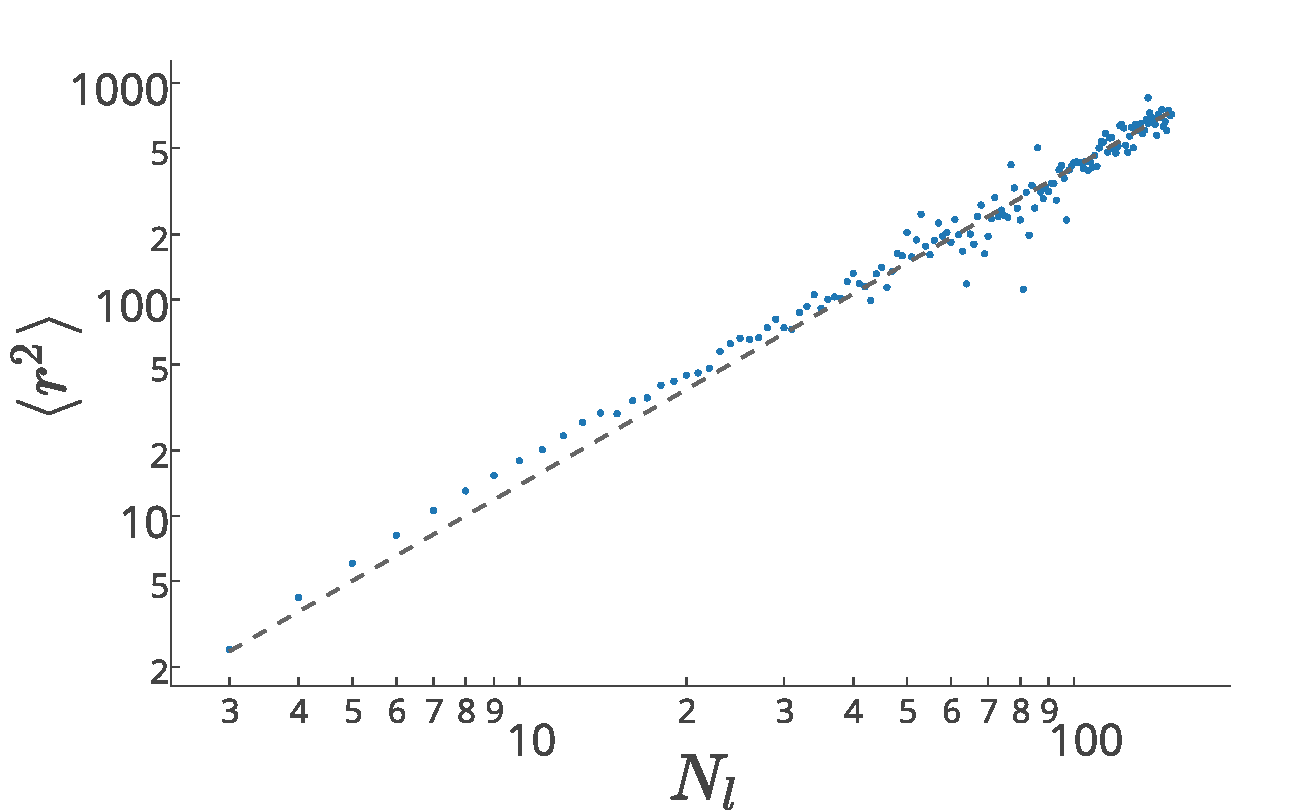
\includegraphics[width=\linewidth]{r_squared.pdf}
    \captionof{figure}{Average end to end distance $\langle r^2\rangle$ as a function of polymer beads $N$ on a log scale. The blue dots depict $\langle r^2\rangle$ and the dashed line is fitted to $\langle r^2\rangle$ with $a\cdot N^{2\nu}$. The fitted value for $2\nu = 1.469 \pm 0.04246$.}
    \label{fig:r_squared}
\end{Figure}


For low temperatures it is expected that the attractive part of the LJ-potential will dominate, causing the polymer to coil up. For higher temperatures, the repulsive part will always dominate, causing the polymer to expand. Since the LJ-potential is negligible beyond a distance of 2.5$\sigma$, the end to end distance will become independent on the temperature for high temperatures. Since a random walk will exhibit an end to end distance $r$ somewhere between these two regimes, it is expected that inbetween the two regimes the temperature $T_c$ can be found where $\langle r^2 \rangle$ equals $\langle r_{random}^2 \rangle$, where $\langle r_{random}^2 \rangle = N$ is the expectation value of the end to end distance squared for a random walk in 2 dimensions.
\begin{Figure}
  \centerfloat
     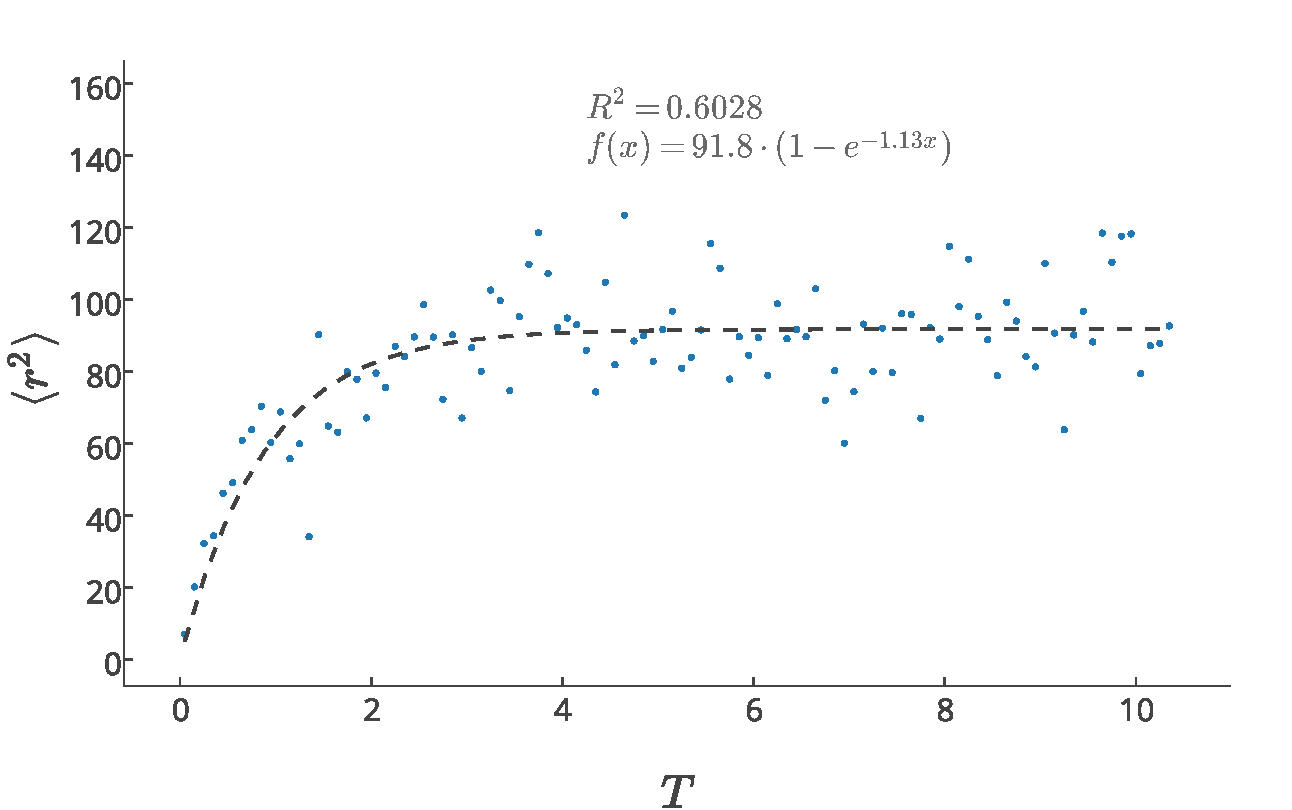
\includegraphics[scale=0.4]{end_to_end_distance_as_function_of_the_temperature.pdf}
 \captionof{figure}{Expectation value for the end to end distance squared as function of the temperature, for polymers with a length of 30 beads}\label{fig:end_to_end_afo_temperature}
\end{Figure} Since for high temperatures $\langle r^2 \rangle$ becomes approximately constant, a fit function in the form of $a(1-e^{-bT})$ was chosen, with $a$ and $b$ the fit parameters. From the fit the value for the critical temperature $T_c$ is found to be approximately 0.35.


\subsection{Bending energy}

As the bending energy parameter $\epsilon_b$ increases, the polymers should straighten out due to straight configurations having a lower energy. At a certain point, the bending energy will overcome the attractive part of the LJ-potential at low temperatures, causing the polymer to uncoil. A simulation was performed where ensembles of 30 beads were generated for $\epsilon_b/k_b$ between 0 and 15 at a temperature of $T = 1$.

\begin{Figure}
  \centerfloat
     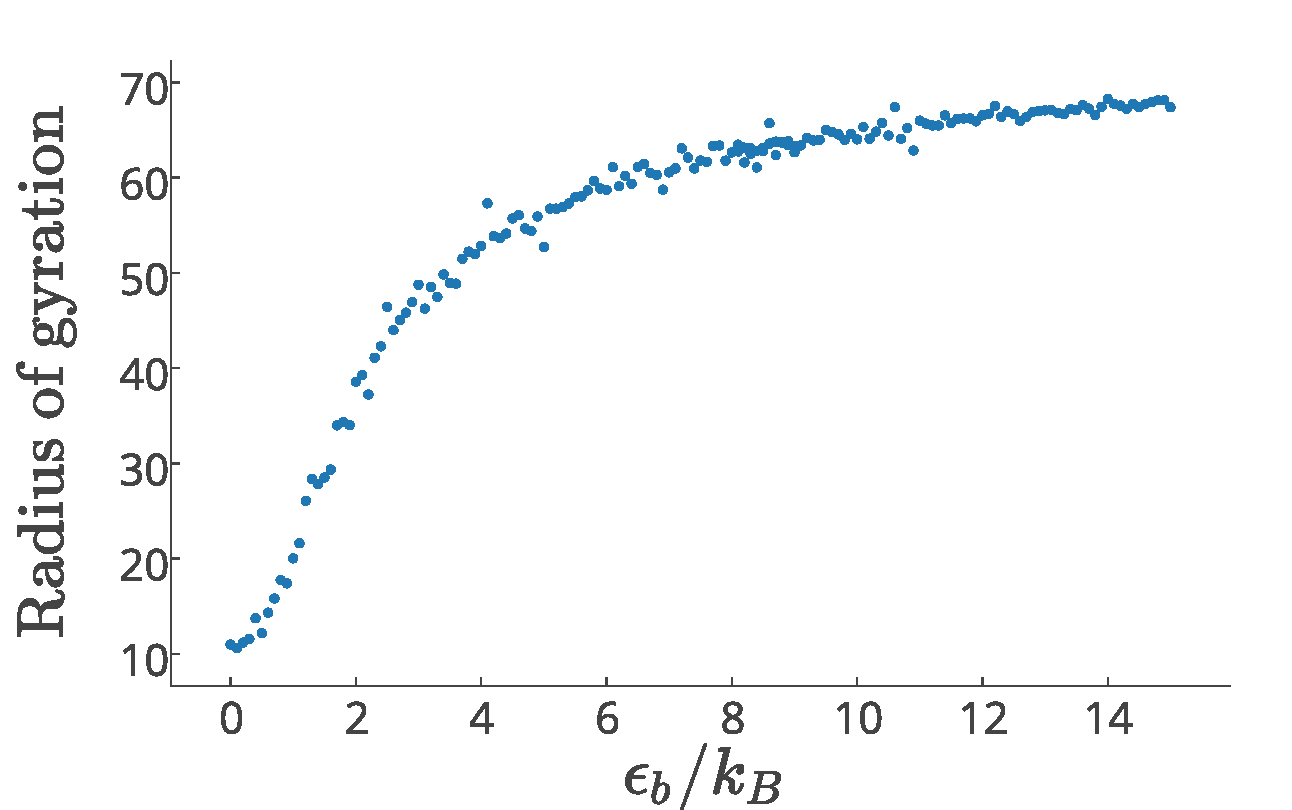
\includegraphics[scale=0.4]{radius_of_gyr_bending.pdf}
 \captionof{figure}{caption}\label{fig:radius_of_gyr_bending}
\end{Figure}

For large values of the bending energy parameter ($\epsilon_b/k_b>6$), the radius of gyration becomes approximately a linear function of $\epsilon_b$. For low values
of the bending energy parameter ($\epsilon_b/k_b<0.5$) the LJ-potential dominates the effects of the system. Between this regime the bending energy overcomes the LJ-potential. In the appendix a similar figure for $\langle r^2\rangle$ can be found.

The fluctuations in $\langle r^2\rangle$ become greater as the polymers get longer. This is most likely due to the fact that the population sizes of the ensembles also fluctuates significantly for larger polymers. This was found to be problem in most of the simulations, and is especially of present for polymers with more than $\sim 40$ beads, where the population size becomes unpredictable. In Figure \ref{fig:r_squared_pop} the population sizes for the ensembles in Figure \ref{fig:r_squared} are depicted. We got the impression that in literature the population size did not fluctuate by large amounts using PERM. Unfortunately we were unable to find the cause of these large fluctuations.

\subsection{Note on the program}
The energy calculations, LJ potential and bending energy, are written in Fortran for better performance. To make a connection between the Fortran code and the Python program, an interface is made using \emph{Fortran to Python interface generator} (F2PY). F2PY creates a Python C/API extension module that makes it possible to call the in Fortran written energy subroutine.